\begin{figure}
\begin{fullpage}
    \begin{center}
        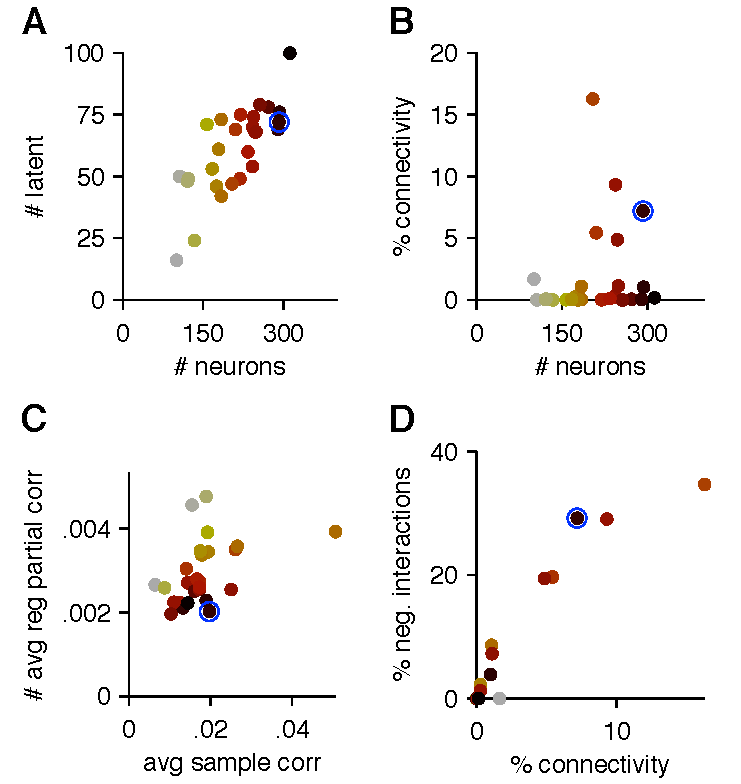
\includegraphics{./figures/Stats.pdf}
    \end{center}

\caption[Properties of functional connectivity across datasets]{
{\bf Properties of functional connectivity across datasets.}
Each point represents an imaged site with its color indicating the population size as shown in panels A and B. The example site from Figures \ref{fig:2} and \ref{fig:4} is circled in blue.
\\
{\bf A.} The number of inferred latent units \emph{vs.}~population size.
{\bf B.} The connectivity of the sparse component of partial correlations as a function of population size.
{\bf C.} The average sample correlations \emph{vs.}~the average partial correlations (Eq.~\ref{eq:partial}) of the $C_{\sf sparse+latent}$ estimate.
{\bf D.} The percentage of negative interactions vs.~connectivity in the $C_{\sf sparse+latent}$ estimates.

}\label{fig:5}

\end{fullpage}
\end{figure}
